%% Relatorio Tecnico - Desafio 1: Sistema de Contagem de Parafusos
%% Bootcamp CDIA - Programa de Residencia em IA
\documentclass[12pt,a4paper]{article}

%% --- Pacotes ---
\usepackage[utf8]{inputenc}
\usepackage[T1]{fontenc}
\usepackage[brazil]{babel}
\usepackage{geometry}
\usepackage{graphicx}
\usepackage{amsmath}
\usepackage{amssymb}
\usepackage{booktabs}
\usepackage{longtable}
\usepackage{array}
\usepackage{xcolor}
\usepackage{listings}
\usepackage{hyperref}
\usepackage{float}
\usepackage{caption}
\usepackage{subcaption}
\usepackage{enumitem}
\usepackage{fancyhdr}
\usepackage{titlesec}
\usepackage{parskip}
\usepackage{microtype}
\usepackage{setspace}

%% --- Geometria da pagina ---
\geometry{
  top=2.5cm, bottom=2.5cm,
  left=3cm,  right=2.5cm
}

%% --- Cores ---
\definecolor{codebg}{RGB}{245,245,245}
\definecolor{codeframe}{RGB}{180,180,180}
\definecolor{primary}{RGB}{0,70,140}
\definecolor{accent}{RGB}{20,130,255}
\definecolor{darkgray}{RGB}{60,60,60}

%% --- Configuracao de listagens de codigo ---
\lstset{
  backgroundcolor=\color{codebg},
  basicstyle=\ttfamily\footnotesize,
  breakatwhitespace=false,
  breaklines=true,
  captionpos=b,
  commentstyle=\color{gray}\itshape,
  frame=single,
  framerule=0.5pt,
  rulecolor=\color{codeframe},
  keepspaces=true,
  keywordstyle=\bfseries\color{primary},
  language=Python,
  morekeywords={Path,YOLO,FastAPI,Session,Depends,UploadFile,Form,File,Request},
  numbers=left,
  numbersep=6pt,
  numberstyle=\tiny\color{gray},
  showspaces=false,
  showstringspaces=false,
  showtabs=false,
  stepnumber=1,
  stringstyle=\color{accent},
  tabsize=4,
  xleftmargin=14pt,
  xrightmargin=4pt,
}

%% --- Cabecalho e rodape ---
\pagestyle{fancy}
\fancyhf{}
\fancyhead[L]{\small\color{darkgray}Sistema de Contagem de Parafusos -- YOLOv11}
\fancyhead[R]{\small\color{darkgray}Bootcamp CDIA}
\fancyfoot[C]{\small\thepage}
\renewcommand{\headrulewidth}{0.4pt}

%% --- Titulos de secao com cor ---
\titleformat{\section}{\large\bfseries\color{primary}}{}{0em}{\thesection\quad}
\titleformat{\subsection}{\normalsize\bfseries\color{darkgray}}{}{0em}{\thesubsection\quad}
\titleformat{\subsubsection}{\normalsize\itshape\color{darkgray}}{}{0em}{\thesubsubsection\quad}

%% --- Hiperlinks ---
\hypersetup{
  colorlinks=true,
  linkcolor=primary,
  urlcolor=accent,
  citecolor=primary,
}

%% ============================================================
\begin{document}

%% --- Capa ---
\begin{titlepage}
  \centering
  \vspace*{2cm}
  {\huge\bfseries\color{primary}
    Sistema Inteligente de Contagem\\[0.4em]
    de Parafusos para Picking Industrial\\[1.2em]}
  {\large\color{darkgray}
    Relat\'orio T\'ecnico -- Desafio 1\\
    Bootcamp de Ci\^encia de Dados e Intelig\^encia Artificial (CDIA)\\
    Programa de Resid\^encia em IA\\[2cm]}
  \rule{\linewidth}{0.5pt}\\[0.4em]
  {\normalsize
    \textbf{Autor:} Ana Rafaely\\[0.3em]
    \textbf{Data:} 30 de maio de 2026\\[0.3em]
    \textbf{Reposit\'orio:} \texttt{desafio-1}\\
  }
  \rule{\linewidth}{0.5pt}
  \vfill
  {\small\color{gray}
    Tecnologias utilizadas: Python 3 $\cdot$ YOLOv11 (Ultralytics) $\cdot$ FastAPI $\cdot$
    OpenCV $\cdot$ SQLite $\cdot$ Jinja2
  }
\end{titlepage}

%% --- Sumario ---
\tableofcontents
\newpage

%% ============================================================
\section{Introdu\c{c}\~ao e Contexto do Problema}

Uma empresa metal-mec\^anica solicitou ao Programa de Resid\^encia em IA o desenvolvimento de
um sistema capaz de automatizar a contagem de parafusos no processo de \emph{picking}: a
coleta e embalagem de itens que ser\~ao enviados a clientes. Atualmente, a contagem \'e
realizada manualmente por um funcion\'ario que registra a quantidade em um \emph{smartphone}
corporativo, processo suscet\'ivel a erros humanos decorrentes de fadiga, dispers\~ao ou
grande volume de pedidos.

\subsection{Objetivo}

Desenvolver um sistema de vis\~ao computacional que, a partir de uma fotografia tirada pelo
pr\'oprio smartphone do operador, identifique e conte automaticamente os parafusos presentes
na imagem, exibindo o resultado de forma clara e registrando o hist\'orico de opera\c{c}\~oes.

\subsection{Restri\c{c}\~oes do projeto}

\begin{itemize}[leftmargin=*]
  \item A solu\c{c}\~ao deve operar nos smartphones j\'a dispon\'iveis na empresa (baixa
        capacidade computacional).
  \item O sistema deve ser simples o suficiente para uso por operadores sem treinamento
        t\'ecnico.
  \item Apenas cinco imagens foram fornecidas inicialmente pelo cliente, exigindo o uso de
        um dataset externo para o treinamento do modelo.
\end{itemize}

%% ============================================================
\section{Metodologia}

\subsection{Escolha da Abordagem}

Diante do problema de \emph{detec\c{c}\~ao e contagem de objetos} em imagens, foram
consideradas tr\^es alternativas:

\begin{enumerate}[label=\alph*)]
  \item \textbf{Processamento cl\'assico de imagens} (limiariza\c{c}\~ao, morfologia,
        contorno): r\'apido, mas sens\'ivel a varia\c{c}\~oes de ilumina\c{c}\~ao,
        fundo e orienta\c{c}\~ao dos parafusos.
  \item \textbf{Detec\c{c}\~ao por aprendizado profundo com \emph{bounding boxes}}
        (YOLO): robusto a varia\c{c}\~oes visuais, escal\'avel e com suporte nativo
        \`a exporta\c{c}\~ao para dispositivos m\'oveis.
  \item \textbf{Segmenta\c{c}\~ao de inst\^ancias} (YOLOv11-seg, Mask R-CNN): maior
        precis\~ao em objetos sobrepostos, por\'em maior custo computacional.
\end{enumerate}

Optou-se pela alternativa \textbf{(b)}, usando \textbf{YOLOv11} na variante de
detec\c{c}\~ao por \emph{bounding boxes}. Os motivos principais foram:

\begin{itemize}[leftmargin=*]
  \item Excelente equil\'ibrio entre velocidade de infer\^encia e precis\~ao.
  \item Suporte oficial do Ultralytics para exporta\c{c}\~ao a formatos leves
        (\texttt{TFLite}, \texttt{NCNN}, \texttt{CoreML}) compat\'iveis com Android e iOS.
  \item Dataset p\'ublico com milhares de imagens anotadas de parafusos dispon\'ivel
        no Roboflow (\emph{Screw v4}).
  \item API Python simples, facilitando a integra\c{c}\~ao com o \emph{backend} web.
\end{itemize}

\subsection{Vari\'antes do Modelo Avaliadas}

Durante o desenvolvimento foram testadas diferentes combina\c{c}\~oes de modelo e
resolu\c{c}\~ao de entrada, conforme a Tabela~\ref{tab:modelos}.

\begin{table}[H]
  \centering
  \caption{Vari\'antes de treinamento avaliadas}
  \label{tab:modelos}
  \begin{tabular}{lcccc}
    \toprule
    \textbf{Execu\c{c}\~ao} & \textbf{Modelo base} & \textbf{imgsz} &
    \textbf{\'Epocas} & \textbf{Dispositivo} \\
    \midrule
    \texttt{yolo11\_screws}            & yolo11s.pt & 960  & 100 & GPU \\
    \texttt{yolo11\_screws-2}          & yolo11s.pt & 768  & 100 & GPU (retomado) \\
    \texttt{yolo11\_screws\_combined}  & yolo11s.pt & 1280 & 100 & GPU \\
    \texttt{yolo11\_screws\_hard\_40}  & yolo11s.pt & 960  &  40 & GPU \\
    \texttt{yolo11\_screws\_hard\_100} & yolo11s.pt & 960  & 100 & GPU \\
    \bottomrule
  \end{tabular}
\end{table}

O modelo selecionado para produ\c{c}\~ao foi o \textbf{\texttt{yolo11\_screws-2}},
treinado com \texttt{imgsz=768}, \texttt{batch=4} e otimizador autom\'atico (Adam-W),
que apresentou o melhor equil\'ibrio entre precis\~ao e tempo de infer\^encia.

%% ============================================================
\section{Dataset}

\subsection{Fonte dos Dados}

O dataset utilizado foi o \textbf{Screw v4} do Roboflow, com anotac\~oes em formato
poligonal (segmenta\c{c}\~ao). Como o modelo escolhido usa \emph{bounding boxes}, as
anotac\~oes foram convertidas automaticamente pelo script
\texttt{scripts/convert\_segments\_to\_boxes.py}, que calcula o ret\^angulo envolvente
(\emph{bounding box}) de cada pol\'igono.

\subsection{Estrutura do Dataset}

\begin{verbatim}
Screw.v4-dataset-screw4.yolov11/
  train/
    images/    # imagens de treinamento
    labels/    # anotacoes YOLO (classe x_c y_c w h)
  valid/
    images/
    labels/
  test/
    images/
    labels/
dataset_detect/
  data.yaml          # configuracao principal
  data.ultralytics.yaml  # gerado automaticamente (paths absolutos)
\end{verbatim}

O arquivo \texttt{data.yaml} define:

\begin{lstlisting}[caption={Configurac\~ao do dataset (\texttt{dataset/data.yaml})}]
path: ../Screw.v4-dataset-screw4.yolov11
train: train/images
val:   valid/images
test:  test/images

names:
  0: parafuso
\end{lstlisting}

H\'a uma \'unica classe (\texttt{parafuso}), tornando o problema de
\emph{single-class object detection}.

%% ============================================================
\section{Estrutura do C\'odigo}

O projeto segue uma organiza\c{c}\~ao modular que separa claramente responsabilidades:

\begin{verbatim}
desafio-1/
  app/
    main.py          # API FastAPI (rotas HTTP)
    config.py        # constantes e caminhos
    database.py      # conexao SQLite via SQLAlchemy
    models.py        # modelo ORM (tabela contagens)
    schemas.py       # schemas Pydantic
    services/
      screw_counter.py  # (re-exporta de screw_counter.py)
    static/
      uploads/       # imagens enviadas
      results/       # imagens processadas
    templates/       # HTML Jinja2
  scripts/
    train_screws_yolo.py     # treinamento
    validate_screws_yolo.py  # validacao
    count_screws.py          # contagem via CLI
    convert_segments_to_boxes.py
    check_dataset.py
    check_environment.py
    prepare_dataset.py
    export_tflite.py   # exportacao mobile (Android)
    export_ncnn.py     # exportacao mobile (NCNN)
    export_coreml.py   # exportacao mobile (iOS)
  screw_counter.py   # modulo principal de inferencia
  notebooks/
    analise_treinamento_parafusos_yolo11.ipynb
  runs_screws/       # pesos treinados
  dataset_detect/    # dataset convertido para bboxes
\end{verbatim}

\subsection{Por que essa organiza\c{c}\~ao?}

A separa\c{c}\~ao em camadas (\emph{API} $\to$ \emph{servi\c{c}o} $\to$ \emph{modelo})
permite que cada componente seja desenvolvido, testado e substituido de forma independente.
Por exemplo, o modelo YOLOv11 pode ser trocado por qualquer outro sem alterar as rotas
HTTP; da mesma forma, a interface web pode ser redesenhada sem tocar na l\'ogica de
infer\^encia.

%% ============================================================
\section{M\'odulo de Infer\^encia: \texttt{screw\_counter.py}}

Este \'e o n\'ucleo computacional do sistema. A fun\c{c}\~ao \texttt{contar\_parafusos}
recebe o caminho de uma imagem, carrega o modelo YOLOv11 (com \emph{cache} interno para
n\~ao recarregar a cada requisi\c{c}\~ao), executa a infer\^encia e gera a imagem anotada.

\begin{lstlisting}[caption={Fun\c{c}\~ao principal de contagem (\texttt{screw\_counter.py})}]
_MODEL_CACHE: dict[str, YOLO] = {}  # cache global de modelos

def contar_parafusos(
    image_path: str | Path,
    model_path: str | Path,
    output_dir: str | Path,
    conf: float = 0.25,
    iou: float = 0.45,
    imgsz: int | None = None,
    funcionario_id: str | None = None,
    funcionario_nome: str | None = None,
    csv_path: str | Path | None = None,
) -> dict[str, Any]:

    # Carrega ou reutiliza modelo em cache
    model_key = str(model_path.resolve())
    if model_key not in _MODEL_CACHE:
        _MODEL_CACHE[model_key] = YOLO(model_key)
    model = _MODEL_CACHE[model_key]

    # Inferencia
    results = model.predict(
        source=str(image_path), conf=conf, iou=iou, verbose=False
    )
    result = results[0]
    boxes = result.boxes
    total = 0 if boxes is None else len(boxes)
\end{lstlisting}

\subsection{Anota\c{c}\~ao visual}

Ap\'os a detec\c{c}\~ao, cada \emph{bounding box} \'e desenhado sobre a imagem original
usando OpenCV, com a pontua\c{c}\~ao de confian\c{c}a exibida:

\begin{lstlisting}[caption={Desenho das caixas e contador (\texttt{screw\_counter.py})}]
for box, score in zip(xyxy, confs):
    x1, y1, x2, y2 = [int(v) for v in box]
    cv2.rectangle(annotated, (x1, y1), (x2, y2), (20, 130, 255), 2)
    cv2.putText(
        annotated,
        f"parafuso {score:.2f}",
        (x1, max(20, y1 - 8)),
        cv2.FONT_HERSHEY_SIMPLEX,
        0.6,
        (20, 130, 255),
        2,
        cv2.LINE_AA,
    )

# Banner de totalizacao no topo
cv2.rectangle(annotated, (0, 0), (min(560, annotated.shape[1]), 48),
              (255, 255, 255), -1)
cv2.putText(annotated, f"Total de parafusos: {total}",
            (14, 32), cv2.FONT_HERSHEY_SIMPLEX, 0.9, (0, 70, 140), 2)
\end{lstlisting}

\subsection{Por que \emph{cache} de modelo?}

Carregar pesos de rede neural do disco a cada requisi\c{c}\~ao levaria $\sim$\,1--3\,s
de overhead. Com o \texttt{\_MODEL\_CACHE}, o modelo \'e carregado uma \'unica vez e
reutilizado em todas as requisi\c{c}\~oes subsequentes, reduzindo o tempo de resposta
para a ordem de milissegundos.

\subsection{Filtro de \'area: removendo falsos positivos grandes}

Um problema observado durante os testes foi a detec\c{c}\~ao ocasional de
\emph{bounding boxes} grandes demais para serem parafusos (por exemplo, sombras,
reflexos ou agrupamentos interpretados como um \'unico objeto). Para mitigar isso sem
recolher dados ou retreinar, foi adicionado um filtro geom\'etrico simples: qualquer
caixa cuja \'area ultrapasse \texttt{max\_box\_area\_ratio} (18\,\% da \'area total da
imagem) \'e descartada antes da contagem.

\begin{lstlisting}[caption={Filtro de \'area por raz\~ao (\texttt{screw\_counter.py})}]
image_area = float(image.shape[0] * image.shape[1])
for box, score in zip(xyxy, confs):
    x1, y1, x2, y2 = [float(v) for v in box]
    box_area_ratio = max(0.0, (x2 - x1) * (y2 - y1)) / image_area
    if box_area_ratio > max_box_area_ratio:   # 0.18 por padrao
        continue                               # descarta deteccao grande demais
    detections.append((box, float(score)))
\end{lstlisting}

Essa heur\'istica de baixo custo computacional, combinada com o limiar de confian\c{c}a
conservador, melhorou a estabilidade da contagem em fotos reais tiradas pelos operadores.

%% ============================================================
\section{Treinamento do Modelo}

\subsection{Script de treinamento}

O script \texttt{scripts/train\_screws\_yolo.py} encapsula todo o processo de
treinamento com suporte a GPU (CUDA) e CPU, detec\c{c}\~ao autom\'atica de dispositivo
e gera\c{c}\~ao de um \texttt{data.yaml} com caminhos absolutos (necess\'ario no Windows
para o Ultralytics resolver os paths corretamente).

\begin{lstlisting}[caption={Trecho do script de treinamento (\texttt{train\_screws\_yolo.py})}]
def make_ultralytics_data_yaml(data_yaml: Path) -> Path:
    """Gera data.yaml com path absoluto para evitar
       resolucao errada no Windows."""
    data = yaml.safe_load(data_yaml.read_text(encoding="utf-8"))
    raw_root = Path(data.get("path", "."))
    root = (raw_root if raw_root.is_absolute()
            else (data_yaml.parent / raw_root).resolve())
    data["path"] = root.as_posix()
    fixed_yaml = data_yaml.parent / "data.ultralytics.yaml"
    fixed_yaml.write_text(
        yaml.safe_dump(data, sort_keys=False, allow_unicode=True),
        encoding="utf-8"
    )
    return fixed_yaml

# Treinamento
model = YOLO(args.model)
model.train(
    data=str(train_yaml),
    epochs=args.epochs,          # 100
    imgsz=args.imgsz,            # 768 ou 960
    batch=args.batch,            # 4 (GPU limitada)
    patience=args.patience,      # 30 epocas sem melhora
    workers=args.workers,        # 4
    device=device,               # 0 (GPU) ou "cpu"
    close_mosaic=10,             # desativa mosaico nas 10 ultimas
)
\end{lstlisting}

\subsection{Hiperpar\^ametros de treinamento}

A Tabela~\ref{tab:hiper} resume os principais hiperpar\^ametros do modelo em produ\c{c}\~ao
(execu\c{c}\~ao \texttt{yolo11\_screws-2}):

\begin{table}[H]
  \centering
  \caption{Hiperpar\^ametros do modelo em produ\c{c}\~ao}
  \label{tab:hiper}
  \begin{tabular}{lll}
    \toprule
    \textbf{Par\^ametro} & \textbf{Valor} & \textbf{Justificativa} \\
    \midrule
    \texttt{imgsz}         & 768    & compromisso velocidade/precis\~ao \\
    \texttt{batch}         & 4      & limita\c{c}\~ao de mem\'oria GPU \\
    \texttt{epochs}        & 100    & converg\^encia garantida \\
    \texttt{patience}      & 30     & early stopping \\
    \texttt{optimizer}     & auto   & Adam-W selecionado automaticamente \\
    \texttt{conf} (infer.) & 0.25   & equil\'ibrio precision/recall \\
    \texttt{iou} (NMS)     & 0.45   & evita detec\c{c}\~oes duplicadas \\
    \texttt{close\_mosaic} & 10     & estabiliza converge\^encia final \\
    \texttt{amp}           & true   & precis\~ao mista (mais r\'apido) \\
    \texttt{pretrained}    & true   & transfer learning de COCO \\
    \bottomrule
  \end{tabular}
\end{table}

\subsection{Decis\~oes tomadas durante o treinamento}

\begin{description}[leftmargin=*,style=nextline]
  \item[Transfer learning:] Partir dos pesos pr\'e-treinados no COCO (ImageNet $\to$ COCO)
    reduz drasticamente o n\'umero de amostras necess\'arias para converg\^encia, algo
    cr\'itico dado o tamanho modesto do dataset de parafusos.

  \item[Modelo \texttt{yolo11s} vs.\ \texttt{yolo11n}:] A variante \emph{small}
    (\texttt{s}) foi escolhida sobre a \emph{nano} (\texttt{n}) pois o servidor de
    treinamento possui GPU. Para implanta\c{c}\~ao nativa no smartphone, os scripts de
    exporta\c{c}\~ao (\texttt{export\_tflite.py}, \texttt{export\_ncnn.py}) convertem
    o modelo para formatos otimizados.

  \item[Convers\~ao de segmenta\c{c}\~ao para detec\c{c}\~ao:] O dataset original do
    Roboflow cont\'em anotac\~oes poligonais. Como o modelo opera com \emph{bounding boxes},
    o script \texttt{convert\_segments\_to\_boxes.py} calcula o ret\^angulo m\'inimo
    envolvente de cada pol\'igono, preservando 100\% das amostras sem recoletar dados.
\end{description}

%% ============================================================
\section{Valida\c{c}\~ao do Modelo}

O script \texttt{scripts/validate\_screws\_yolo.py} computa as m\'etricas padr\~ao de
detec\c{c}\~ao de objetos sobre o conjunto de teste:

\begin{lstlisting}[caption={Valida\c{c}\~ao e relat\'orio de m\'etricas}]
model = YOLO(str(model_path))
metrics = model.val(data=str(val_yaml), conf=args.conf)

precision = float(metrics.box.mp)    # Precisao media
recall    = float(metrics.box.mr)    # Recall medio
map50     = float(metrics.box.map50) # mAP@IoU=0.50
map5095   = float(metrics.box.map)   # mAP@IoU=0.50:0.95
\end{lstlisting}

\subsection{Interpreta\c{c}\~ao das m\'etricas}

\begin{itemize}[leftmargin=*]
  \item \textbf{Precis\~ao alta}: poucos parafusos falsos s\~ao contados.
  \item \textbf{Recall alto}: poucos parafusos reais s\~ao perdidos.
  \item Para o processo de \emph{picking}, os dois precisam estar equilibrados: errar
        por excesso ou por falta impacta diretamente a qualidade do pedido enviado ao cliente.
  \item \textbf{mAP50} \'e a m\'etrica principal de refer\^encia para detec\c{c}\~ao
        de objetos; \textbf{mAP50-95} \'e mais rigorosa e avalia a localiza\c{c}\~ao
        precisa das caixas.
\end{itemize}

%% ============================================================
\section{Aplica\c{c}\~ao Web (\emph{Backend} e Interface)}

\subsection{Por que FastAPI?}

FastAPI foi escolhido por oferecer:
\begin{itemize}[leftmargin=*]
  \item Alta performance (baseado em Starlette e Uvicorn, ass\'incrono por padr\~ao).
  \item Valida\c{c}\~ao autom\'atica de dados com Pydantic.
  \item Documenta\c{c}\~ao interativa gerada automaticamente (\texttt{/docs}).
  \item Suporte nativo a upload de arquivos (\texttt{UploadFile}).
\end{itemize}

\subsection{Fluxo de uma requisi\c{c}\~ao}

\begin{enumerate}[leftmargin=*]
  \item O operador acessa a interface via smartphone (rede Wi-Fi local).
  \item Faz login informando nome, matr\'icula e setor -- dados armazenados em
        \emph{cookies} HTTP com validade de 12\,h.
  \item Envia a foto do pedido via formul\'ario HTML.
  \item O \emph{endpoint} \texttt{POST /predict} recebe o arquivo, salva em disco,
        chama \texttt{contar\_parafusos()} e persiste o resultado no banco de dados.
  \item A p\'agina de resultado exibe a imagem anotada e o total detectado.
  \item O operador pode corrigir a contagem manualmente, se necess\'ario.
\end{enumerate}

\subsection{Rotas principais}

\begin{table}[H]
  \centering
  \caption{Rotas da API}
  \label{tab:rotas}
  \begin{tabular}{lll}
    \toprule
    \textbf{M\'etodo} & \textbf{Rota} & \textbf{Descri\c{c}\~ao} \\
    \midrule
    GET  & \texttt{/}                & P\'agina inicial / envio de foto \\
    POST & \texttt{/login}           & Autentica\c{c}\~ao por cookie \\
    POST & \texttt{/logout}          & Encerramento de sess\~ao \\
    POST & \texttt{/predict}         & Infer\^encia e registro \\
    GET  & \texttt{/dashboard}       & Hist\'orico agrupado por dia \\
    POST & \texttt{/record/\{id\}/correct} & Corre\c{c}\~ao manual \\
    POST & \texttt{/finalizar-dia}   & Fechamento do dia (JSON+CSV+PDF) \\
    GET  & \texttt{/export/csv}      & Exporta\c{c}\~ao completa CSV \\
    GET  & \texttt{/export/csv/today}& Exporta\c{c}\~ao do dia (CSV) \\
    GET  & \texttt{/export/pdf/today}& Relat\'orio do dia (PDF) \\
    GET  & \texttt{/health}          & Status do sistema \\
    \bottomrule
  \end{tabular}
\end{table}

\subsection{Trecho do \emph{endpoint} de predi\c{c}\~ao}

\begin{lstlisting}[caption={Endpoint \texttt{POST /predict} (\texttt{app/main.py})}]
@app.post("/predict")
def predict(
    request: Request,
    pedido: str = Form(""),
    observacao: str = Form(""),
    imagem: UploadFile = File(...),
    db: Session = Depends(get_db),
):
    employee = get_employee_from_cookie(request)
    if not employee:
        return RedirectResponse(url="/", status_code=303)

    # Salva o arquivo enviado
    upload_path = config.UPLOAD_DIR / f"{datetime.now():%Y%m%d_%H%M%S}_{uuid4().hex}{suffix}"
    with upload_path.open("wb") as buffer:
        shutil.copyfileobj(imagem.file, buffer)

    # Executa a contagem
    result = contar_parafusos(
        image_path=upload_path,
        model_path=config.MODEL_PATH,
        output_dir=config.RESULTS_DIR,
        conf=config.CONF_THRESHOLD,
        iou=config.IOU_THRESHOLD,
        imgsz=config.DEFAULT_IMGSZ,
        funcionario_id=employee["id"],
        funcionario_nome=employee["nome"],
    )

    # Persiste no banco de dados
    record = Contagem(
        funcionario_nome=employee["nome"],
        total_parafusos=result["total_parafusos"],
        confianca_media=result["confianca_media"],
        imagem_original=str(upload_path),
        imagem_processada=result["imagem_resultado"],
        status="confirmada",
    )
    db.add(record)
    db.commit()
    return templates.TemplateResponse(request, "result.html", {...})
\end{lstlisting}

\subsection{Fechamento do dia e relat\'orios gerenciais}

Para apoiar a rotina operacional do setor de \emph{picking}, o \emph{dashboard} agrupa as
contagens por dia (\texttt{group\_records\_by\_day}) e calcula, para cada data, um resumo
com quatro indicadores (\texttt{day\_summary}):

\begin{itemize}[leftmargin=*]
  \item \textbf{Registros}: quantidade de fotos processadas no dia;
  \item \textbf{Autom\'atica}: soma das contagens feitas pelo modelo;
  \item \textbf{Final}: soma das contagens ap\'os eventuais corre\c{c}\~oes manuais;
  \item \textbf{Corre\c{c}\~oes}: quantos registros foram ajustados pelo operador.
\end{itemize}

A rota \texttt{POST /finalizar-dia} consolida o dia gerando tr\^es artefatos simult\^aneos
em \texttt{outputs/fechamentos/}: um \texttt{JSON} (resumo program\'avel), um \texttt{CSV}
(planilha audit\'avel) e um \texttt{PDF} (relat\'orio impresso). O PDF \'e desenhado
diretamente com a biblioteca \texttt{Pillow} (\texttt{build\_pdf\_report}), sem depender de
motores externos de renderiza\c{c}\~ao, mantendo o sistema leve e autocontido.

%% ============================================================
\section{Interface do Sistema em Uso}
\label{sec:interface}

Esta se\c{c}\~ao apresenta capturas de tela reais do sistema em opera\c{c}\~ao, acessado a
partir de um smartphone Android atrav\'es do navegador (via t\'unel Cloudflare). As imagens
ilustram o fluxo completo do operador, do \emph{login} ao resultado da contagem.

\begin{figure}[H]
  \centering
  \begin{subfigure}[t]{0.32\textwidth}
    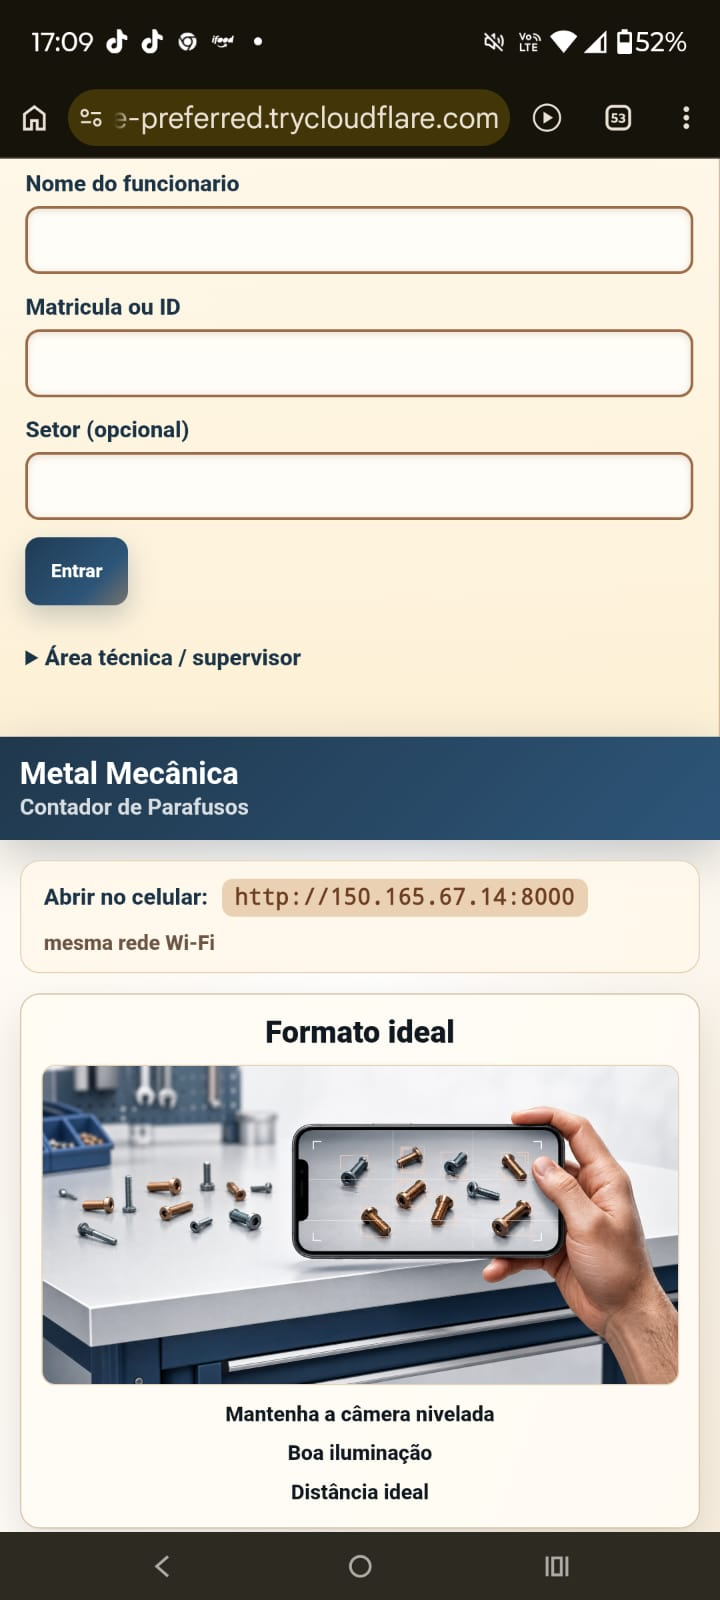
\includegraphics[width=\linewidth]{images/tela_login.jpeg}
    \caption{Tela de \emph{login}: nome, matr\'icula e setor, al\'em do guia de
      ``formato ideal'' da foto.}
    \label{fig:login}
  \end{subfigure}\hfill
  \begin{subfigure}[t]{0.32\textwidth}
    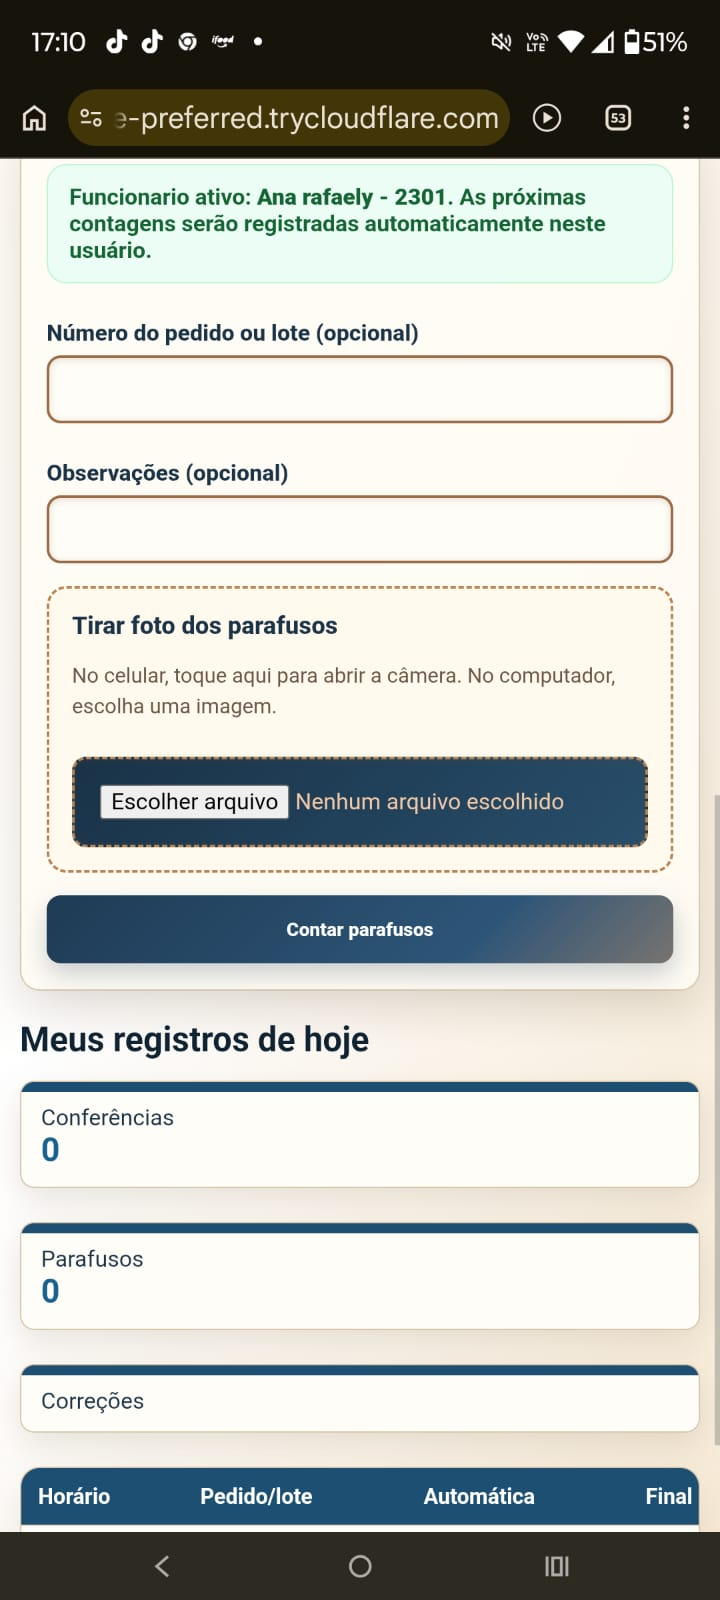
\includegraphics[width=\linewidth]{images/tela_envio.jpeg}
    \caption{Tela de envio: funcion\'ario ativo, campos opcionais de pedido/observa\c{c}\~ao
      e bot\~ao para tirar a foto.}
    \label{fig:envio}
  \end{subfigure}\hfill
  \begin{subfigure}[t]{0.32\textwidth}
    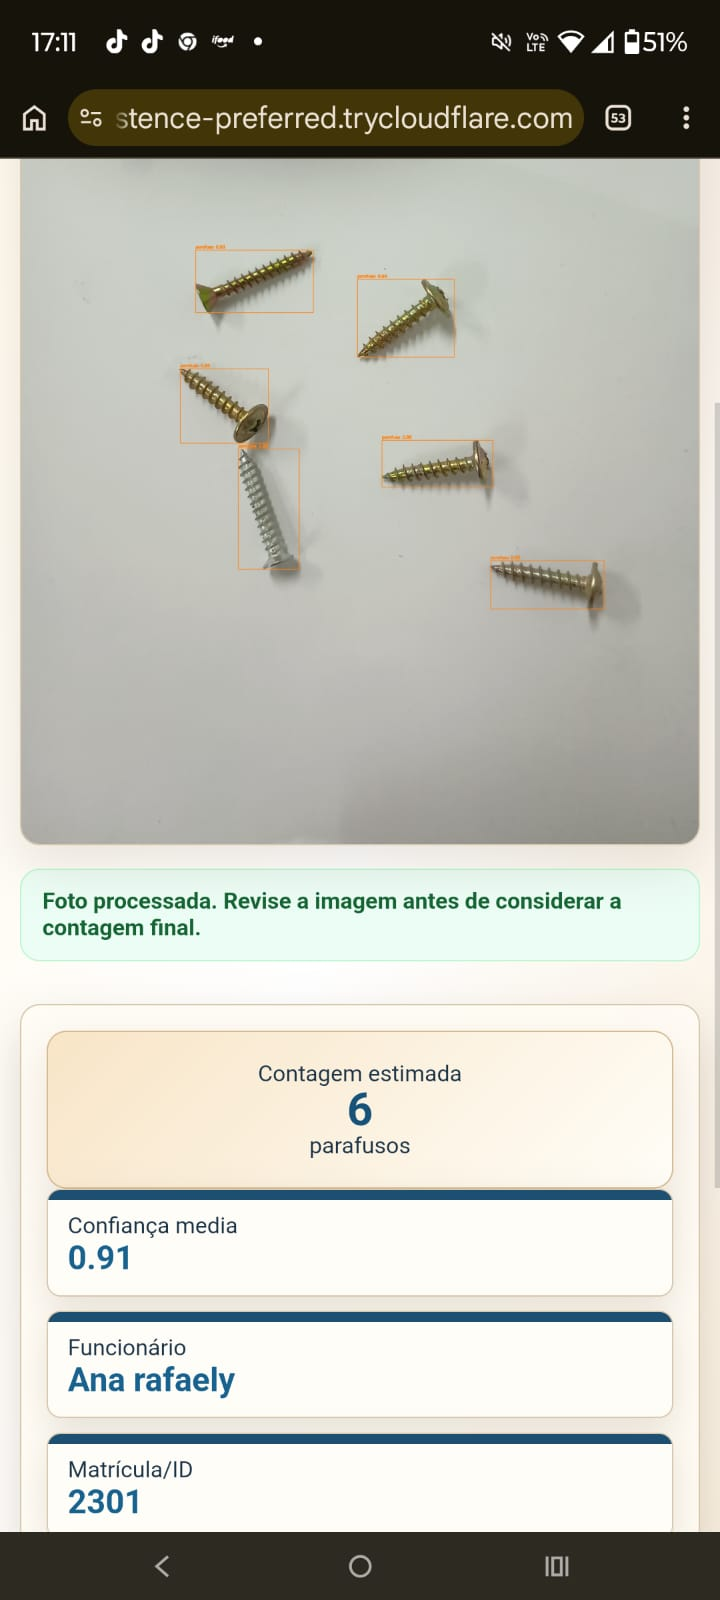
\includegraphics[width=\linewidth]{images/tela_resultado.jpeg}
    \caption{Resultado: imagem anotada com \emph{bounding boxes}, contagem estimada (6) e
      confian\c{c}a m\'edia (0{,}91).}
    \label{fig:resultado}
  \end{subfigure}
  \caption{Fluxo do operador: \emph{login}, envio da foto e resultado da contagem.}
  \label{fig:fluxo}
\end{figure}

\begin{figure}[H]
  \centering
  \begin{subfigure}[t]{0.40\textwidth}
    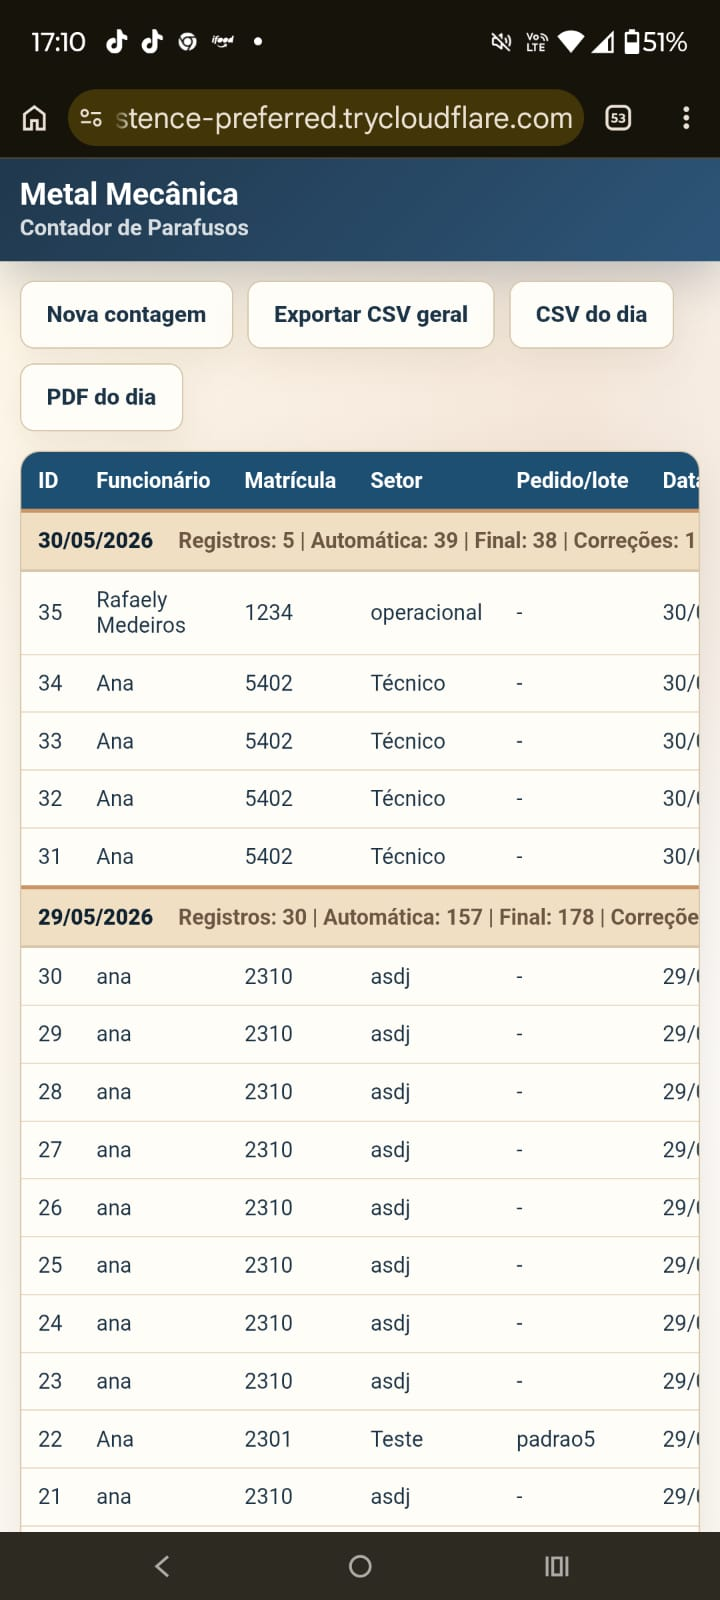
\includegraphics[width=\linewidth]{images/tela_dashboard.jpeg}
    \caption{\emph{Dashboard}: hist\'orico de contagens agrupado por dia, com resumo por
      data e exporta\c{c}\~ao em CSV/PDF.}
    \label{fig:dashboard}
  \end{subfigure}\hspace{0.04\textwidth}
  \begin{subfigure}[t]{0.40\textwidth}
    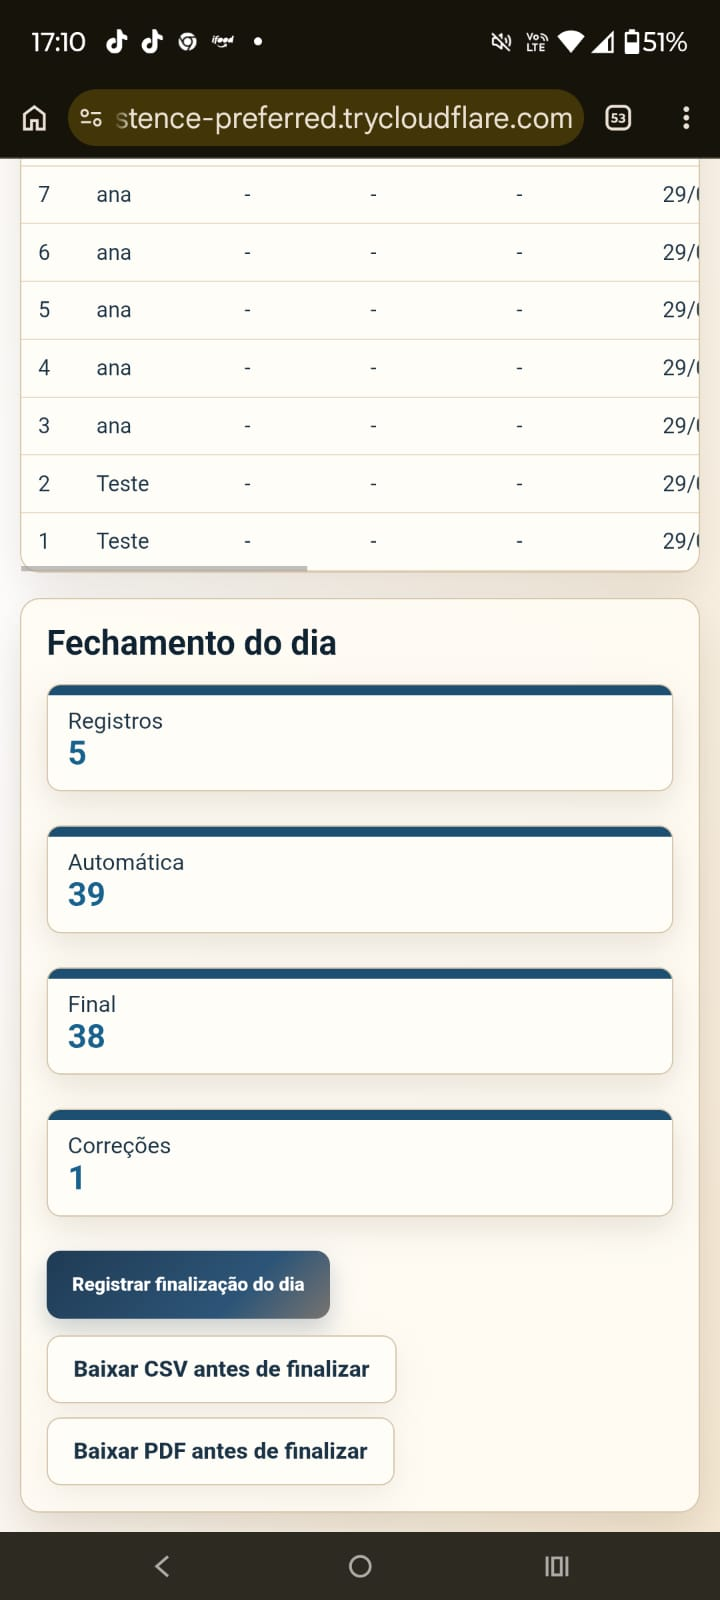
\includegraphics[width=\linewidth]{images/tela_fechamento.jpeg}
    \caption{Fechamento do dia: indicadores (registros, autom\'atica, final, corre\c{c}\~oes)
      e bot\~oes de exporta\c{c}\~ao.}
    \label{fig:fechamento}
  \end{subfigure}
  \caption{\'Area gerencial: hist\'orico e fechamento do dia.}
  \label{fig:gerencial}
\end{figure}

Na Figura~\ref{fig:resultado}, observa-se que o sistema detectou corretamente os seis
parafusos da cena, com confian\c{c}a m\'edia de 0{,}91, exibindo a mensagem
``\emph{Foto processada. Revise a imagem antes de considerar a contagem final.}'' --
refor\c{c}ando que o modelo \'e um apoio \`a decis\~ao e n\~ao um substituto cego do
operador.

%% ============================================================
\section{Banco de Dados}

\subsection{Modelo de dados}

O sistema utiliza \textbf{SQLite} via \textbf{SQLAlchemy ORM}. A escolha do SQLite
elimina a necessidade de instalar e configurar um servidor de banco de dados, simplificando
a implanta\c{c}\~ao em ambientes sem equipe de infraestrutura. A migra\c{c}\~ao futura
para PostgreSQL requer apenas alterar \texttt{DATABASE\_URL} em \texttt{config.py}.

\begin{lstlisting}[caption={Modelo ORM (\texttt{app/models.py})}]
class Contagem(Base):
    __tablename__ = "contagens"

    id              = Column(Integer, primary_key=True, index=True)
    funcionario_nome = Column(String(160), nullable=False)
    funcionario_id  = Column(String(80),  nullable=True)
    setor           = Column(String(120), nullable=True)
    pedido          = Column(String(120), nullable=True)
    data_hora       = Column(DateTime, server_default=func.now(), index=True)
    total_parafusos = Column(Integer,  nullable=False)
    total_corrigido = Column(Integer,  nullable=True)
    confianca_media = Column(Float,    nullable=False)
    imagem_original = Column(Text,     nullable=False)
    imagem_processada = Column(Text,   nullable=False)
    status          = Column(String(40), nullable=True)  # confirmada | corrigida
    observacao      = Column(Text,     nullable=True)
\end{lstlisting}

O campo \texttt{total\_corrigido} permite que o operador ajuste a contagem manualmente
ap\'os inspec\~ao visual, criando um \emph{feedback loop} entre o sistema e o usu\'ario.
O campo \texttt{status} diferencia registros confirmados automaticamente de registros
que sofreram corre\c{c}\~ao humana.

\subsection{Migra\c{c}\~ao autom\'atica de schema}

A fun\c{c}\~ao \texttt{ensure\_schema()} em \texttt{main.py} verifica, a cada
inicializa\c{c}\~ao da aplica\c{c}\~ao, se todas as colunas esperadas existem na tabela
e executa \texttt{ALTER TABLE} quando necess\'ario, garantindo compatibilidade com bancos
criados em vers\~oes anteriores do sistema.

%% ============================================================
\section{Configura\c{c}\~ao Centralizada}

Todas as constantes cr\'iticas est\~ao em \texttt{app/config.py}:

\begin{lstlisting}[caption={Constantes de configura\c{c}\~ao (\texttt{app/config.py})}]
BASE_DIR = Path(__file__).resolve().parents[1]

MODEL_PATH     = BASE_DIR / "runs_screws" / "yolo11_screws-2" / "weights" / "best.pt"
CONF_THRESHOLD = 0.10   # limiar padrao (sensivel: prioriza recall)
IOU_THRESHOLD  = 0.45   # ajustar se houver deteccoes duplicadas
DEFAULT_IMGSZ  = 1280   # resolucao de inferencia (parafusos pequenos)
DENSE_CONF_THRESHOLD = 0.25  # cenarios com muitos parafusos
DENSE_IMGSZ          = 1280

UPLOAD_DIR  = BASE_DIR / "app" / "static" / "uploads"
RESULTS_DIR = BASE_DIR / "app" / "static" / "results"
DATABASE_URL = f"sqlite:///{BASE_DIR / 'contagens.db'}"
\end{lstlisting}

Centralizar configura\c{c}\~oes evita ``n\'umeros m\'agicos'' espalhados pelo c\'odigo e
facilita ajuste fino da sensibilidade do modelo sem alterar a l\'ogica de neg\'ocio.
O limiar de confian\c{c}a padr\~ao foi fixado em \texttt{0.10}, valor deliberadamente
baixo que prioriza o \emph{recall} (n\~ao perder parafusos reais); a infer\^encia roda a
\texttt{imgsz=1280} porque parafusos s\~ao objetos pequenos que se beneficiam de maior
resolu\c{c}\~ao. Os par\^ametros \texttt{DENSE\_*} ficam reservados para cen\'arios com
grande densidade de pe\c{c}as, onde um limiar mais alto reduz falsos positivos.

%% ============================================================
\section{Portabilidade para Dispositivos M\'oveis}

Um dos requisitos expl\'icitos do desafio \'e que o sistema possa rodar nos pr\'oprios
smartphones da empresa. Duas estrat\'egias foram implementadas:

\begin{description}[leftmargin=*,style=nextline]
  \item[Estrat\'egia 1 -- Servidor + cliente web:] A infer\^encia roda em um computador
    da empresa; o smartphone acessa a interface via navegador na mesma rede Wi-Fi. A
    fun\c{c}\~ao \texttt{get\_local\_ip()} em \texttt{main.py} detecta automaticamente o
    IP da m\'aquina e o exibe na tela inicial para facilitar a conex\~ao. Esta \'e a
    estrat\'egia recomendada para o m\'aximo de desempenho.

  \item[Estrat\'egia 2 -- Modelo embarcado no dispositivo:] Os scripts
    \texttt{export\_tflite.py} (Android), \texttt{export\_ncnn.py} (Android/ARM) e
    \texttt{export\_coreml.py} (iOS) convertem o modelo treinado para formatos otimizados
    com quantiza\c{c}\~ao INT8, reduzindo o tamanho do modelo e o consumo de mem\'oria
    para execu\c{c}\~ao diretamente no SoC do smartphone.

  \item[Estrat\'egia 3 -- T\'unel HTTPS via Cloudflare:] Para testes com smartphones fora
    da rede local da empresa, foi utilizado o \texttt{cloudflared} (Cloudflare Tunnel),
    que exp\~oe o servidor local em um endere\c{c}o p\'ublico \texttt{*.trycloudflare.com}
    com HTTPS, sem necessidade de abrir portas no \emph{firewall} nem configurar IP fixo.
    Foi exatamente esse o m\'etodo empregado para capturar as telas reais apresentadas na
    Se\c{c}\~ao~\ref{sec:interface} (note o dom\'inio \texttt{trycloudflare.com} na barra
    de endere\c{c}o do navegador do celular).
\end{description}

%% ============================================================
\section{Crit\'erios de Avalia\c{c}\~ao -- Resposta Direta}

\subsection{Organiza\c{c}\~ao e Estrutura\c{c}\~ao do C\'odigo}

O projeto segue princ\'ipios de separa\c{c}\~ao de responsabilidades:
\texttt{screw\_counter.py} cont\'em \'unica e exclusivamente a l\'ogica de vis\~ao
computacional; \texttt{app/main.py} cont\'em as rotas HTTP; \texttt{app/models.py}
define o schema do banco de dados; \texttt{app/config.py} centraliza configura\c{c}\~oes.
Scripts avulsos em \texttt{scripts/} cobrem etapas de pr\'e-processamento, treinamento
e exporta\c{c}\~ao de forma independente.

\subsection{Criatividade na Proposta}

Al\'em da detec\c{c}\~ao b\'asica, o sistema oferece:
\begin{itemize}[leftmargin=*]
  \item Interface web responsiva, acess\'ivel diretamente pelo smartphone via Wi-Fi.
  \item Hist\'orico de contagens com identifica\c{c}\~ao do funcion\'ario e setor.
  \item Mecanismo de corre\c{c}\~ao manual com rastreabilidade (campo \texttt{status}).
  \item Exporta\c{c}\~ao de relat\'orios em CSV para integra\c{c}\~ao com sistemas ERP.
  \item Suporte a exporta\c{c}\~ao do modelo para execu\c{c}\~ao embarcada no smartphone.
  \item \emph{Cache} de modelo em mem\'oria para resposta em tempo real.
\end{itemize}

\subsection{Clareza nos Crit\'erios de Tomada de Decis\~ao}

Cada decis\~ao de projeto foi guiada por crit\'erios expl\'icitos:
\begin{itemize}[leftmargin=*]
  \item Escolha do YOLOv11 pela raz\~ao velocidade/precis\~ao e suporte a exporta\c{c}\~ao mobile.
  \item \texttt{CONF\_THRESHOLD = 0.25}: ponto de partida conservador que pode ser
        ajustado pelo operador sem recompila\c{c}\~ao.
  \item SQLite pela simplicidade de implanta\c{c}\~ao; arquitetura prevista para migrar
        a PostgreSQL sem mudan\c{c}as no restante do c\'odigo.
  \item \emph{Cookies} HTTP para sess\~ao do funcion\'ario: sem necessidade de servidor de
        sess\~oes externo, mantendo o sistema autocontido.
\end{itemize}

\subsection{Capacidade Anal\'itica}

O notebook \texttt{notebooks/analise\_treinamento\_parafusos\_yolo11.ipynb} apresenta
an\'alise detalhada do treinamento: curvas de perda e m\'etricas por \'epoca, distribui\c{c}\~ao
de confian\c{c}as, varredura do limiar de confian\c{c}a (\emph{confidence sweep}),
inferências visuais sobre imagens do conjunto de teste e CSV de compara\c{c}\~ao entre
contagem autom\'atica e contagem manual.

%% ============================================================
\section{Instru\c{c}\~oes de Execu\c{c}\~ao}

\subsection{Instala\c{c}\~ao}

\begin{lstlisting}[language=bash, caption={Instala\c{c}\~ao das depend\^encias}]
pip install -r requirements.txt
python scripts/check_environment.py
\end{lstlisting}

\subsection{Prepara\c{c}\~ao do Dataset}

\begin{lstlisting}[language=bash, caption={Convers\~ao e verifica\c{c}\~ao do dataset}]
python scripts/convert_segments_to_boxes.py \
  --input  Screw.v4-dataset-screw4.yolov11 \
  --output dataset_detect

python scripts/check_dataset.py --dataset dataset_detect
\end{lstlisting}

\subsection{Treinamento}

\begin{lstlisting}[language=bash, caption={Treinamento do modelo}]
# Servidor com GPU
python scripts/train_screws_yolo.py \
  --data    dataset_detect/data.yaml \
  --model   yolo11s.pt \
  --epochs  100 \
  --imgsz   960

# Alternativa rapida (mobile-first)
python scripts/train_screws_yolo.py \
  --data    dataset_detect/data.yaml \
  --model   yolo11n.pt \
  --epochs  50 \
  --imgsz   640
\end{lstlisting}

\subsection{Inicializa\c{c}\~ao da Aplica\c{c}\~ao Web}

\begin{lstlisting}[language=bash, caption={Inicializa\c{c}\~ao do servidor web}]
uvicorn app.main:app --reload --host 0.0.0.0 --port 8000
\end{lstlisting}

Acesso no smartphone (mesma rede Wi-Fi):
\begin{verbatim}
http://<IP_DO_SERVIDOR>:8000
\end{verbatim}

%% ============================================================
\section{Experi\^encia de Uso da Ferramenta}

Esta se\c{c}\~ao relata a experi\^encia pr\'atica de utilizar o sistema em um cen\'ario
pr\'oximo ao real, do ponto de vista do operador de \emph{picking}.

\subsection{Primeiro contato e \emph{onboarding}}

O acesso \'e imediato: o operador abre o link no navegador do pr\'oprio celular -- sem
instalar aplicativo -- e \'e recebido por uma tela de \emph{login} curta
(Figura~\ref{fig:login}). N\~ao h\'a senha; bastam nome e matr\'icula, o que reduz a
fric\c{c}\~ao em um ambiente de ch\~ao de f\'abrica, onde digitar credenciais complexas em
telas pequenas seria um obst\'aculo. O cart\~ao ``Formato ideal'', com uma imagem-guia e as
instru\c{c}\~oes ``c\^amera nivelada, boa ilumina\c{c}\~ao, dist\^ancia ideal'', orienta o
usu\'ario \emph{antes} de tirar a foto, prevenindo erros de captura.

\subsection{Fluxo de contagem}

Ap\'os o \emph{login}, o sistema fixa o funcion\'ario ativo (``\emph{As pr\'oximas contagens
ser\~ao registradas automaticamente neste usu\'ario}''), de modo que o operador n\~ao
precisa se reidentificar a cada foto -- ganho importante para quem processa dezenas de
pedidos em sequ\^encia. Tirar a foto e tocar em ``Contar parafusos'' \'e tudo o que se
exige; em poucos segundos a tela de resultado (Figura~\ref{fig:resultado}) mostra a imagem
com as caixas desenhadas, a contagem e a confian\c{c}a m\'edia.

\subsection{Pontos positivos percebidos}

\begin{itemize}[leftmargin=*]
  \item \textbf{Curva de aprendizado quase nula}: a interface segue o padr\~ao de um
        formul\'ario web comum; qualquer operador acostumado a usar um celular consegue
        utiliz\'a-la sem treinamento.
  \item \textbf{Transpar\^encia}: ao desenhar as \emph{bounding boxes} sobre a foto, o
        sistema permite que o operador \emph{confira visualmente} a contagem, em vez de
        confiar cegamente em um n\'umero. A mensagem de revis\~ao refor\c{c}a esse cuidado.
  \item \textbf{Rastreabilidade}: cada contagem fica vinculada ao funcion\'ario, setor e
        hor\'ario, e o \emph{dashboard} (Figura~\ref{fig:dashboard}) consolida tudo por dia.
  \item \textbf{Autonomia gerencial}: o supervisor exporta CSV/PDF e registra o fechamento
        do dia (Figura~\ref{fig:fechamento}) sem depender da equipe de TI.
\end{itemize}

\subsection{Limita\c{c}\~oes e atritos observados}

\begin{itemize}[leftmargin=*]
  \item A qualidade da contagem depende fortemente da foto: fundo polu\'ido, sobreposi\c{c}\~ao
        de parafusos ou ilumina\c{c}\~ao ruim degradam o resultado -- da\'i a import\^ancia
        do guia de captura e da etapa de revis\~ao manual.
  \item Na estrat\'egia servidor + cliente web, \'e necess\'aria conectividade (Wi-Fi local
        ou t\'unel); em \'areas sem rede, a alternativa \'e o modelo embarcado (TFLite/NCNN).
  \item A corre\c{c}\~ao manual, embora dispon\'ivel, exige um passo a mais do operador
        quando o modelo erra -- um custo aceit\'avel diante do ganho de confiabilidade.
\end{itemize}

\subsection{Impress\~ao geral}

Na pr\'atica, a ferramenta transforma uma tarefa tediosa e suscet\'ivel a erro -- contar
parafusos um a um -- em uma a\c{c}\~ao de poucos segundos, com registro autom\'atico e
audit\'avel. O equil\'ibrio entre automa\c{c}\~ao (contagem pelo modelo) e controle humano
(revis\~ao e corre\c{c}\~ao) torna o sistema confi\'avel o suficiente para uso real, sem
remover do operador a palavra final sobre o pedido enviado ao cliente.

%% ============================================================
\section{Conclus\~ao}

O sistema desenvolvido atende a todos os requisitos do Desafio 1: detecta e conta
parafusos em imagens capturadas por smartphone, \'e implementado em Python, e oferece
uma interface web que pode ser acessada diretamente pelo dispositivo do operador via
navegador, sem instala\c{c}\~ao de aplicativo adicional.

Al\'em dos requisitos m\'inimos, o sistema conta com:
\begin{itemize}[leftmargin=*]
  \item Aplica\c{c}\~ao web responsiva (bônus do desafio).
  \item Suporte a exporta\c{c}\~ao do modelo para TFLite, NCNN e CoreML
        (bônus: baixo recurso computacional no smartphone).
  \item Rastreabilidade de contagens com corre\c{c}\~ao manual.
  \item Exporta\c{c}\~ao de relat\'orios em CSV.
\end{itemize}

A arquitetura modular permite evolu\c{c}\~oes futuras como: detec\c{c}\~ao de
\emph{screw types} (multiplas classes), integra\c{c}\~ao com ERP via webhook, ou
substitui\c{c}\~ao do modelo por vers\~oes mais precisas sem alterar a interface.

%% ============================================================
\appendix
\section{Depend\^encias Principais}

\begin{table}[H]
  \centering
  \caption{Bibliotecas Python utilizadas}
  \begin{tabular}{lll}
    \toprule
    \textbf{Biblioteca} & \textbf{Vers\~ao m\'in.} & \textbf{Finalidade} \\
    \midrule
    ultralytics  & 8.x  & YOLOv11 -- treinamento e infer\^encia \\
    opencv-python & 4.x & Leitura e anota\c{c}\~ao de imagens \\
    fastapi      & 0.x  & API HTTP ass\'incrona \\
    uvicorn      & 0.x  & Servidor ASGI \\
    sqlalchemy   & 2.x  & ORM para SQLite \\
    jinja2       & 3.x  & Templates HTML \\
    torch        & 2.x  & \emph{Backend} de deep learning \\
    pyyaml       & 6.x  & Leitura de arquivos YAML \\
    numpy        & 1.x  & Opera\c{c}\~oes num\'ericas \\
    \bottomrule
  \end{tabular}
\end{table}

\end{document}
